\documentclass[aps,prl,reprint]{revtex4-1}
\usepackage{blindtext}

\usepackage{amsmath}
\usepackage{graphicx}
\usepackage{commath}

\usepackage[b]{esvect}

\newcommand{\de}{\mathrm{d}}

\begin{document}
\title{Homework 1}
\author{Xueqi Li}
\noaffiliation
% \date{Feb 4, 2017}
% \email{xueqi.li@stonybrook.edu}

\begin{abstract}
Consider a vector (given with respect to a fixed Cartesian basis). Here $t$ means time.
\[
\vv{r}(t) = \sin(\pi t)\hat{x} + \cos(\pi t)\hat{y} - \sqrt{7}\hat{z}
\]
\end{abstract}

\maketitle

\begin{enumerate}
\item Problem 1
\begin{enumerate}
\item Find the length of $\vv{r}(t)$
\begin{eqnarray*}
    \norm{\vv{r}(t)} & = & \sqrt{\sin^2\pi t + \cos^2\pi t + (-\sqrt{7})^2}  \\
     & = & \sqrt{1+7} \\
     & = & \sqrt{8}
\end{eqnarray*}
\item Find $\vv{r} \cdot \vv{w}$ where $\vv{w} = \hat{x} -2\hat{y}+\sqrt{7}\hat{z}$
\begin{eqnarray*}
    \vv{r} \cdot \vv{w} &=& (\sin\pi t , \cos\pi t ,- \sqrt{7}) \cdot (1,-2,\sqrt{7})\\
    &=& (\sin\pi t, -2\cos{\pi t}, -7)
\end{eqnarray*}
\item Find $\vv{r} \times \vv{w}$
\begin{eqnarray*}
    \vv{r} \times \vv{w} &=&
        \begin{vmatrix}
            \hat{\imath} & \hat{\jmath} & \hat{k} \\
            \sin\pi t & \cos\pi t & - \sqrt{7} \\
            1 & 2 & \sqrt{7}
    \end{vmatrix} \\
    &=& (\sqrt{7}\cos\pi t + 2\sqrt{7},-\sqrt{7}\sin\pi t +\sqrt{7}, \sqrt{7}\sin\pi t + \sqrt{7} )
\end{eqnarray*}
\end{enumerate}
\item Problem 2
\begin{enumerate}
\item Find $\vv{v}(t) = \frac{\mathrm{d}\vv{r}}{\mathrm{d}t}$
\begin{eqnarray*}
\vv{v}(t) &=& \frac{\mathrm{d}\vv{r}}{\mathrm{d}t} \\
&=& (\pi\cos\pi t, -\pi \sin\pi t, 0)
\end{eqnarray*}
\item What is the second derivative?
\begin{eqnarray*}
\ddot{\vv{r}} &=& \frac{\de}{\de t} \vv{v}(t) \\
&=& (-\pi^2\sin\pi t, -\pi^2 \cos\pi t, 0)
\end{eqnarray*}
\end{enumerate}
\item Sketch the trajectory of the vector $\vv{r}(t)$. What kind of a shape does it sweep out?
\begin{center}
 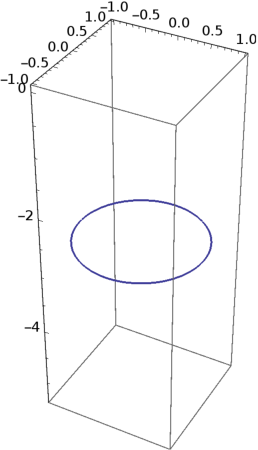
\includegraphics[height=2.5in]{plot1.pdf}
\end{center}
It is a circle.
\item Suppose that $\vv{r}(t)$ describes the motion of a body with mass $m$
\begin{enumerate}
\item Find the momentum.
\[
\vv{p} = m\vv{v} = (\pi m \cos\pi t, -\pi m \sin\pi t, 0)
\]
\item Find the force that is needed to make it move along the path.
\[
\vv{F} = m\ddot{\vv{r}} = (-\pi^2 m \sin\pi t, -\pi^2 m \cos\pi t, 0)
\]
\end{enumerate}
\item Problem 5
\begin{enumerate}
\item Write $\vv{r}(t)$ in a sylindrical cordinate basis
Clear it is a circle at a plane where $z = 0$. Thus we can write
\[
(r, \theta, z) = (1, \tan^{-1}(\frac{\cos\pi t}{\sin \pi t}), -\sqrt{7})
\]
we can also find out that it should be
\begin{eqnarray*}
\begin{bmatrix}
    r\\
    \theta \\
    z
\end{bmatrix}
&=&
\begin{bmatrix}
    \cos\theta & \sin\theta & 0\\
    -\sin\theta & \cos\theta & 0 \\
    0 & 0 & 1
\end{bmatrix}
\begin{bmatrix}
    \sin\pi t\\
    \cos\pi t \\
    -\sqrt{7}
\end{bmatrix} \\
&=&
\begin{bmatrix}
    \sin\pi t \cos\theta + \cos\pi t \sin\theta\\
    -\sin\pi t \sin\theta + \cos\theta \cos\pi t \\
    -\sqrt{7}
\end{bmatrix} \\
\end{eqnarray*}
% where now we can find taht $r = 1 = \sin\pi t \cos\theta + \cos\pi t \sin\theta$. Therefore we can solve $\theta$ by making $\cos\theta = \sin\pi t = \cos(\pi t + \frac{3}{2}\pi)$ and $\sin\theta = \cos\pi t = \sin(\pi t + \frac{1}{2}\pi)$. We can find that $\theta = \pi t + \frac{2}{3}\pi$ just a solution.
where now we can find that $r = 1 = \sin\pi t \cos\theta + \cos\pi t \sin\theta = \sin(\pi t \theta)$. Solve this equation we can find that $\theta = 2\pi n - \pi t + \frac{1}{2} \pi$. Take $n = 0$ we can have $\theta = -\pi t + \frac{1}{2}\pi$. 
% Now we can plug it into $-\sin\pi t \sin\theta + \cos\theta \cos\pi t$, which give us $\theta = 0$. Thus we can have $(r,\theta, z) = (1,0,-\sqrt{7})$
\item What is the time derivative $\frac{\de \hat{r}}{\de t}$ for this motion?
\begin{eqnarray*}
\frac{\de}{\de t}\hat{r} &=& \cos\theta(t) \hat{x} + \sin\theta(t) \hat{y}\\
&=& -\frac{\de \theta(t)}{\de t} \sin\theta(t) \hat{x} + \frac{\de \theta(t)}{\de t} \cos\theta(t) \hat{y} \\
&=& \frac{\de \theta(t)}{\de t} (\cos\theta \hat{y} - \sin\theta\hat{x}) \\
&=& \frac{\de \theta(t)}{\de t} \hat{\theta}
\end{eqnarray*}
\item Compute the first derivative in a cylindrical coordinate basis.
% \begin{eqnarray*}
% \frac{\de}{\de t}\vv{r} &=& \frac{\de}{\de t}\hat{r}  \frac{\de}{\de t}\hat{\theta} \\
% &=& \frac{\de}{\de t}\theta \hat{\theta} \\
% &=& \frac{\de}{\de t}(-\pi t + \frac{1}{2}\pi) \hat{\theta} \\
% &=& -\pi \hat{\theta}
% \end{eqnarray*}
% \begin{eqnarray*}
% \frac{\de}{\de t}\vv{r} &=& \frac{\de}{\de t}\hat{r} + \frac{\de}{\de t}(-\pi t + \frac{1}{2}\pi)\hat{\theta} \\
% &=& \frac{\de}{\de t}\theta \hat{\theta} -\pi t + \frac{\de}{\de t}\hat{\theta}\\
% &=& \frac{\de}{\de t}(-\pi t + \frac{1}{2}\pi) \hat{\theta} \\
% &=& -\pi \hat{\theta}
% \end{eqnarray*}
\begin{eqnarray*}
\frac{\de}{\de t}\vv{r} &=& \dot{r}\hat{r} + r \dot{\theta}\hat{\theta} \\
&=& -r\pi t \hat{\theta}\\
&=& -\pi t \hat{\theta}
\end{eqnarray*}
The Problem 2 give $\dot{\vv{r}} = \pi \cos\pi t \hat{x} - \pi \sin \pi t \hat{y}$. And we can transform it into cylindrical cordinate. 
We can have 
 $r = \sqrt{\pi^2 \cos^2\pi t + \pi^2 \sin^2 \pi t} = \pi$, 
 $\theta = \tan^{-1}(-\frac{\pi \sin \pi t}{\pi \cos \pi t}) = -\pi t$ and $z = 0$ which is agree with the answer above.
\end{enumerate}
\item Problem 6
\begin{enumerate}
\item Compute the length of $\vv{p}(t)$
\begin{eqnarray*}
\norm{\vv{p}(t)} &=& \sqrt{(\pi m \cos\pi t)^2+ (-\pi m \sin\pi t)^2}\\
&=& \sqrt{\pi^2m^2} = \pi m 
\end{eqnarray*}
\item Compute $\hat{z}\cdot(\vv{r}\times\vv{p})$
\begin{eqnarray*}
\hat{z}\cdot(\vv{r}\times\vv{p}) &=& \hat{z}\cdot
        \begin{vmatrix}
            \hat{\imath} & \hat{\jmath} & \hat{k} \\
            \sin\pi t & \cos\pi t & - \sqrt{7} \\
            \pi m \cos\pi t & -\pi m \sin\pi t & 0
    \end{vmatrix} \\
% &=& \hat{k} \cdot (-\pi m \sqrt{7}\sin\pi t, \pi m \sqrt{7}\cos\pi t, -\pi m \sin^2\pi t-\pi m \cos^2 \pi t)\\
&=& \hat{k} \cdot (\cdots, \cdots, -\pi m \sin^2\pi t-\pi m \cos^2 \pi t)\\
&=& \hat{k} \cdot (\cdots, \cdots, -\pi m)\\
&=& (0,0,-\pi m) 
\end{eqnarray*}
\end{enumerate}
\end{enumerate}





%\begin{center}
% 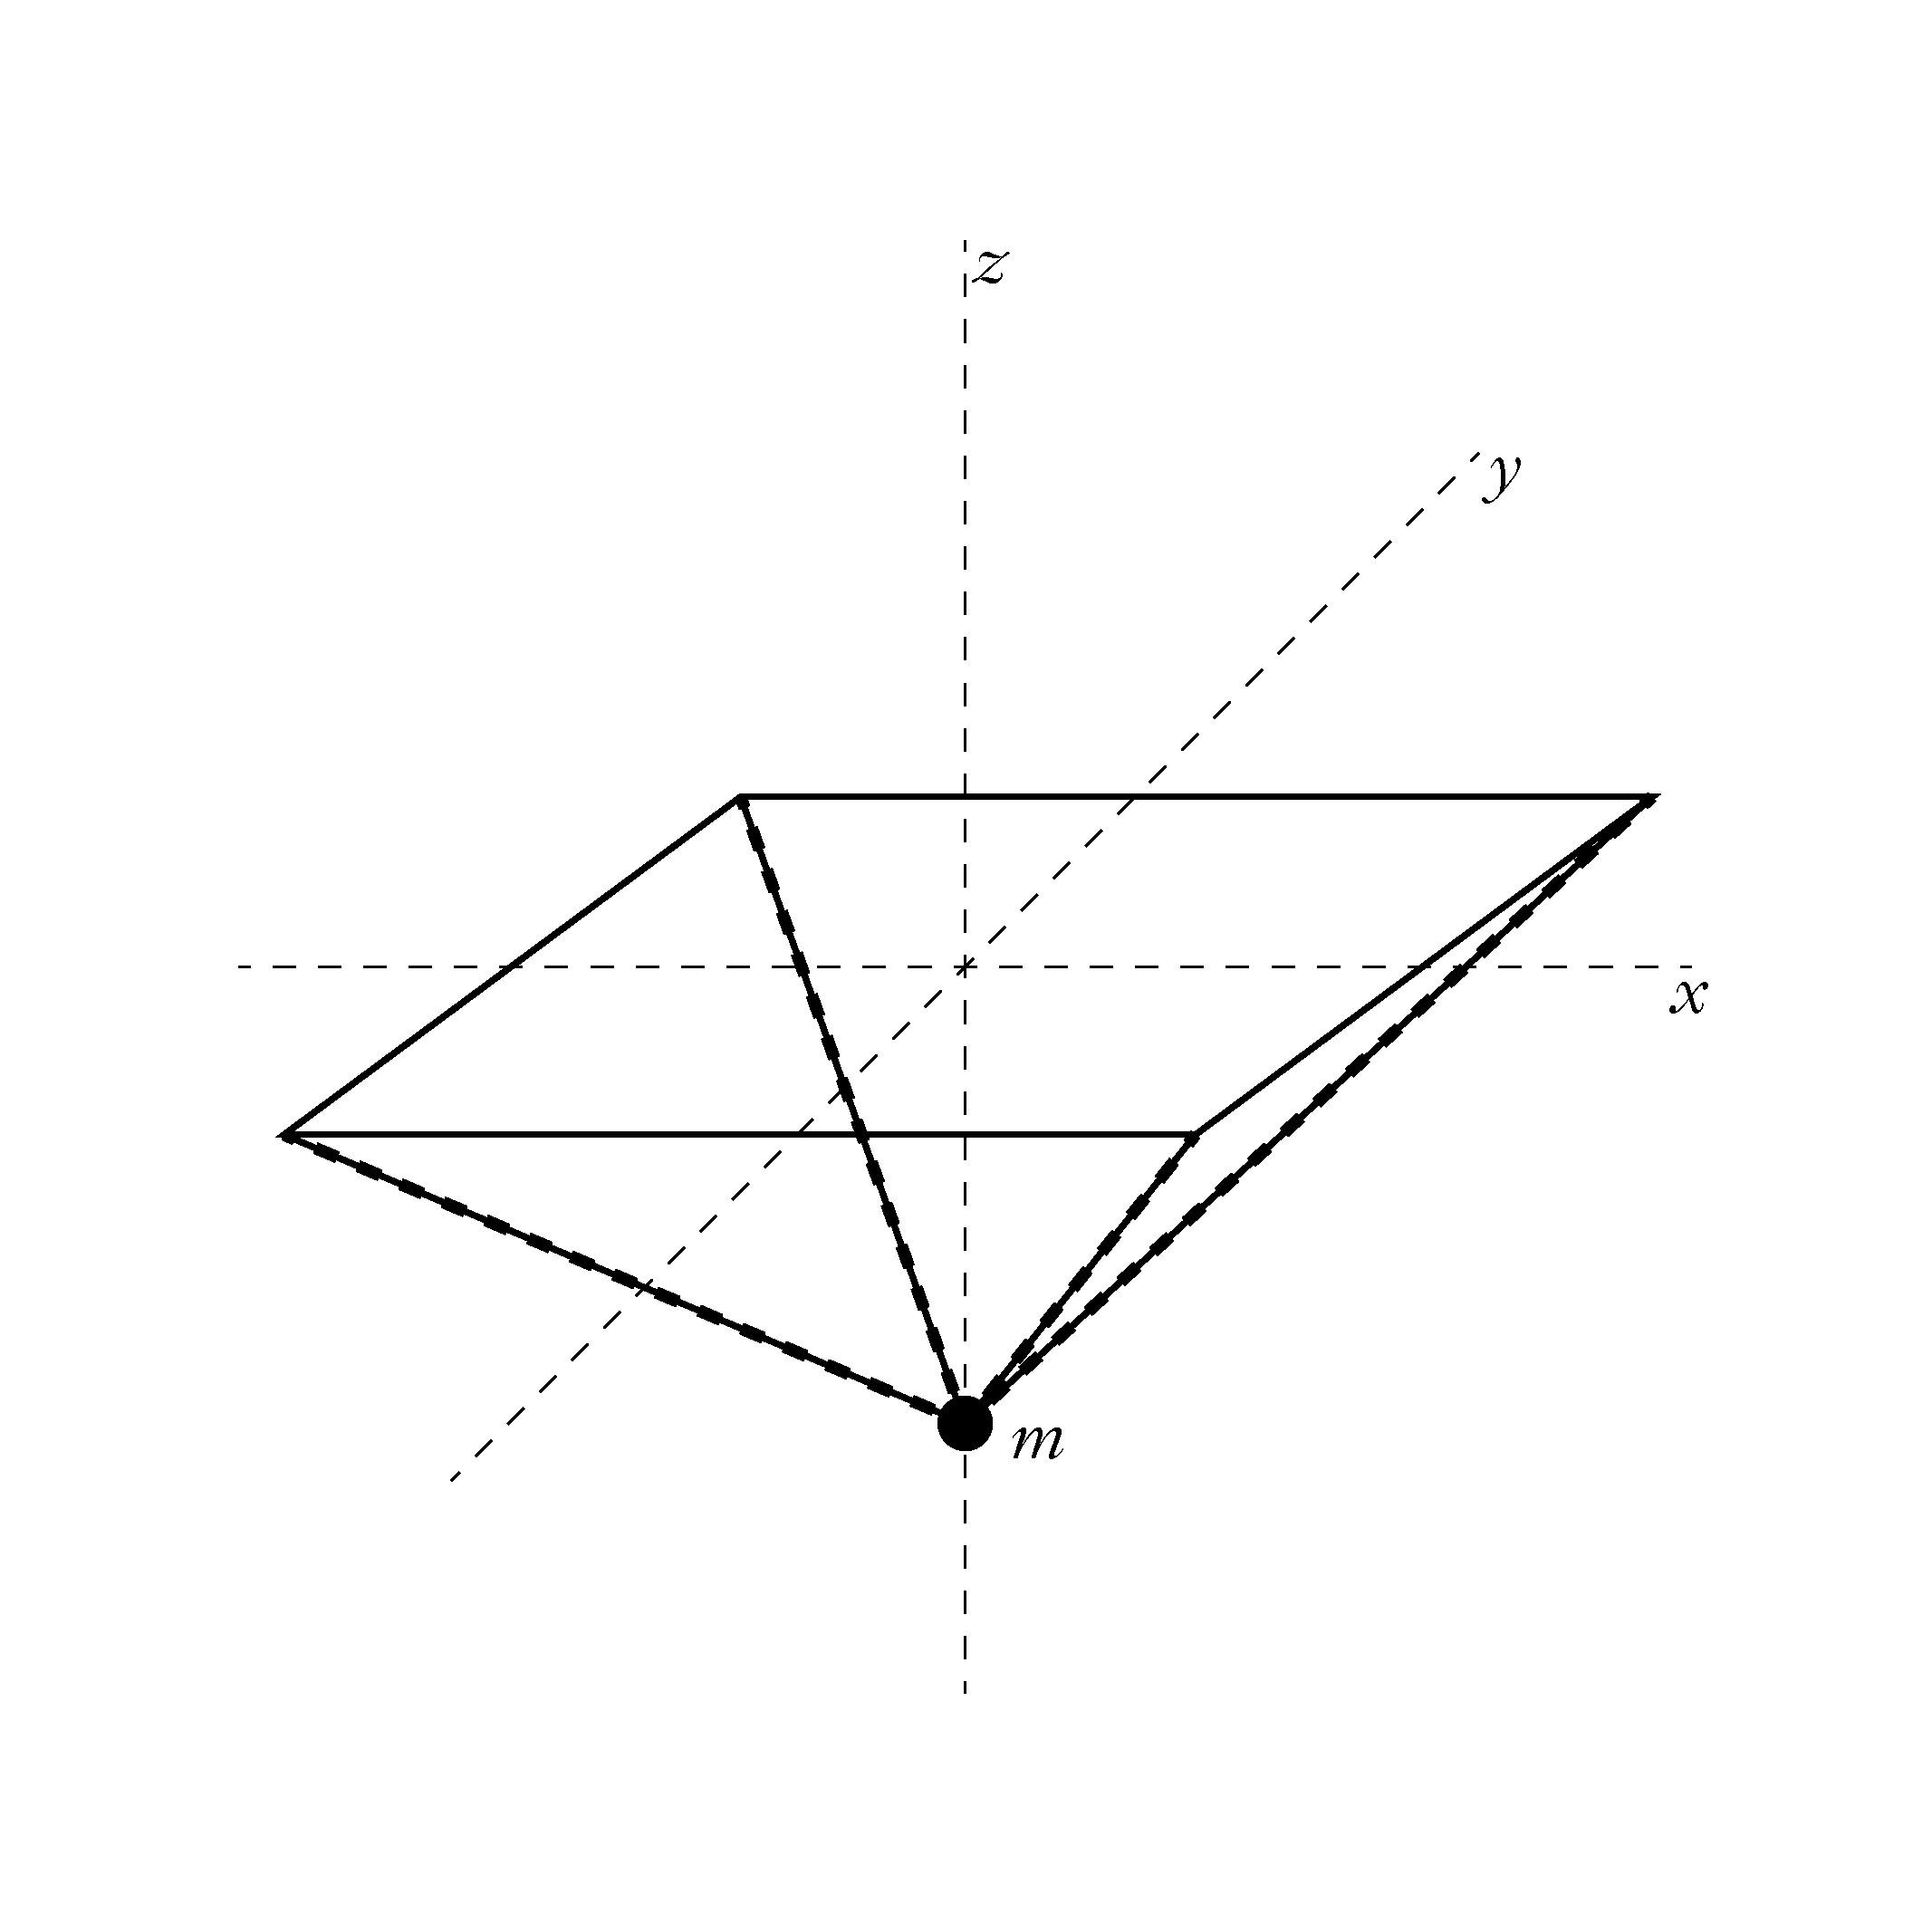
\includegraphics[height=1.3in]{plot.pdf}
%\end{center}

% \blindtext \cite{article-minimal}

% \bibliographystyle{apsrev4-1} % Tell bibtex which bibliography style to use
% \bibliography{xampl} % Tell bibtex which .bib file to use (this one is some example file in TexLive's file tree)

\end{document}